\section{Esfera celeste}

Para aplicação no rastreador estelar, as estrelas são representadas através de uma esfera celeste, na  qual as estrelas são distribuídas em uma esfera ao redor do centro, que na aplicação de satélites é a própria Terra. 
Devido a diferença de escalas da distância das estrelas da Terra, e o tamanho da Terra, 
pode-se considerar que qualquer ponto na Terra e na órbita terrestre, estão exatamente no centro da esfera. 
O erro gerado por tal simplificação só se tornaria visível em missões em que o veículo espacial se retirasse do sistema solar, o que não é caso para Cubesats atuais \cite{Fialho}.

Também é completamente desprezado qualquer movimento que os astros tenham em relação uns aos outros, 
pois estes movimentos são praticamente nulos em nossas análises.
Isto se deve o fato de que, o quanto maior for a distância do observador a um objeto, 
menor será a variação angular para um mesmo movimento linear do objeto, 
como por exemplo pode-se observar que aviões aparentam estar extremamente lento para um observador na Terra, 
No caso do sistema estrelar, esse efeito é ainda maior, permitindo desprezar esse movimento relativo entre as estrelas sem nenhum prejuízo prático a precisão ~\cite[]{Carvalho}.

Nesta abordagem, algumas das características da Terra são representadas na esfera, como o eixo de rotação em torno de si (rotação) e os pólos geográficos, 
que são nomeados respectivamente eixo e pólos celestes. Com isto, facilita-se a localização dos astro na esfera. 
Para isto cria-se circunferências envolvendo a esfera, concorrendo nos polos (meridianos), 
com circunferências perpendiculares ao eixo de rotação (paralelos) ~\cite[]{Carvalho}.

\begin{figure}[H]
	\centering
	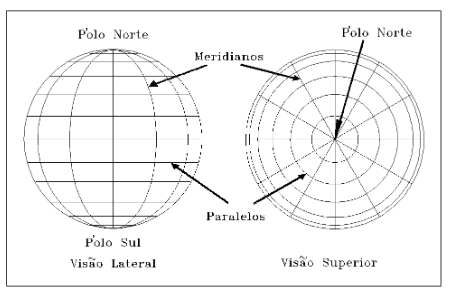
\includegraphics[width=.7\columnwidth]{images/codficacao_cod_esferas_celetes.png}
	\caption{Codificação de coordenadas na esfera celeste. Fonte: ~\cite[]{Carvalho}}
	\label{fig:codficacao_cod_esferas_celetes}
\end{figure}

Como referência tem-se o paralelo central, conhecido como paralelo do Equador,  o meridiano de referência é o que contém o ponto vernal . O ponto vernal é o momento em que o Sol passa o Equador de Sul para Norte, isto ocorre pois a rotação da Terra em torno do próprio eixo está inclinada em relação ao plano da trajetória elíptica da Terra em torno do Sol.Como é visto na Figura  ~\ref{fig:inclinacao}.

\begin{figure}[H]
	\centering
	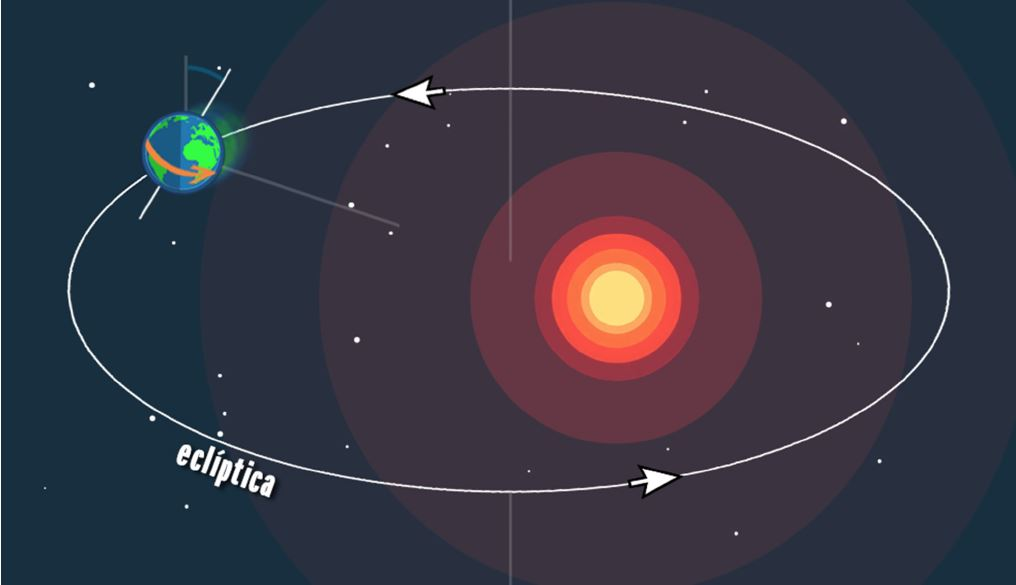
\includegraphics[width=.7\columnwidth]{images/inclinacao.jpg}
	\caption{Inclinação órbita terrestre. Fonte: ~\cite[]{Portal_do_Astronomo}}
	\label{fig:inclinacao}
\end{figure}

